% Intended LaTeX compiler: pdflatex
\documentclass[10pt,a4paper,UTF8]{article}
\usepackage{zclorg}
\date{}
\title{练习:子空间,和与直和}
\hypersetup{
 pdfauthor={},
 pdftitle={练习:子空间,和与直和},
 pdfkeywords={},
 pdfsubject={},
 pdfcreator={Emacs 25.0.50.1 (Org mode 9.0.5)}, 
 pdflang={English}}
\begin{document}

\maketitle
\tableofcontents
\titlepic{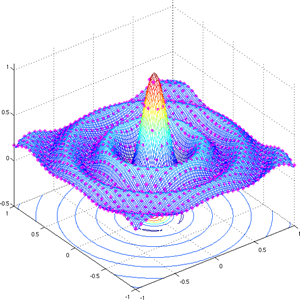
\includegraphics[scale=0.25]{../../img/sinc.PNG}}

\section*{1.c.1}
\label{sec:org0c989e6}

\begin{problem}
1.C.1 判断 \(\mathbf{F}^{3}\)的下列子集是不是\(\mathbf{F}^{3}\)的子空间
\begin{enumerate}
\item \label{orgcfdd0be} \(U=\{(x_{1},x_{2},x_{3})\in \mathbf{F}^{3}: x_{1} + 2x_{2} + 3x_{3} = 0\}\)
\item \label{orga1a8fae} \(V=\{(x_{1},x_{2},x_{3})\in \mathbf{F}^{3}: x_{1} + 2x_{2} + 3x_{3} = 4\}\)
\item \label{orgb355b8a} \(W=\{(x_{1},x_{2},x_{3})\in \mathbf{F}^{3}: x_{1} x_{2}x_{3} = 0\}\)
\item \label{org8d51ca5} \(Z=\{(x_{1},x_{2},x_{3})\in \mathbf{F}^{3}: x_{1}  = 5x_{3}\}\)
\end{enumerate}
\end{problem}

\begin{answer}
针对这个简单的问题,我们只需要按照子空间判断的三个条件来一一确认即可:
\(V\)的子集\(U\)是\(V\)的子空间当且仅当\(U\)满足以下三个条件:

\begin{enumerate}
\item 加法单位元 \(0\in U\);
\item 加法封闭性 : \(u,w\in U \rightarrow u+w\in U\);
\item 标量乘法封闭性:\(a\in \mathbf{F}, u\in U \rightarrow au\in U\)
\end{enumerate}

对于\hyperref[orgcfdd0be]{第一个问题} ,显然有\((0,0,0)\in \mathbf{F}^{3}\)也在\(U=\{(x_{1},x_{2},x_{3})\in \mathbf{F}^{3}: x_{1} + 2x_{2} + 3x_{3} = 0\}\)中。

对于可加性,设\((x,y,z)\in U,(u,v,w)\in U\),则有\(x+2y +3z = 0, u+2v+3w =0\),进而有\((x+u) + 2(y+v) + 3(z+w) = 0\),即\((x+u,y+v,z+w)\in U\)

对于齐次性,设\((x,y,z)\in U\),则有\(\lambda(x+2y+3z) = 0\),进而有\(\lambda x + 2(\lambda y) + 3(\lambda z) = 0\),即,\((\lambda x,\lambda y,\lambda z)\in U\)

综上\(\{(x_{1},x_{2},x_{3})\in \mathbf{F}^{3}: x_{1} + 2x_{2} + 3x_{3} = 0\}\)是\(\mathbf{F}^{3}\)的子空间.

对于\hyperref[orga1a8fae]{第二个问题},显然\((0,0,0)\in \mathbf{F}^{3}\),但是\((0,0,0)\notin V\) ,还可以验证这个子空间不满足齐次可加性。

对于\hyperref[orgb355b8a]{第三个问题},\((0,0,0)\in \mathbf{F}^{3}\)且\((0,0,0)\in W\),但是\((1,1,0)\in W\),\((1,0,1)\in W\) \((1,1,0) + (1,0,1) = (2,1,1)\notin W\)

对于\hyperref[org8d51ca5]{第四个问题},假设\((x,y,z)\in Z, (u,v,w)\in Z\),则有\(x=5c,z=5w\),所以\((x+u)=5z + 5w=5(z+w)\),所以\((x+u,y+v,z+w)\in Z\), 

对于齐次性: \(\lambda \in \mathbf{F}\),\((a,b,c)\in W\),则有\(\lambda a = \lambda (5c) = 5(\lambda c)\),即\((\lambda a,\lambda b,\lambda c)\in Z\)
\end{answer}
\section*{1.c.3}
\label{sec:org56ebf14}


\begin{problem}
1.C.3 证明区间\((-4,4)\)上满足\(f^{'}(-1) = 3f(2)\)的可微实值函数\(f\)构成的集合是\(\mathbf{R}^{(-4,4)}\)的子空间。
\end{problem}

\begin{answer}
首先指定加法单位元是定义如下的函数\(0:(-4,4)\rightarrow \mathbf{R}\),对所有的\(x\in (-4,4)\)都有\(0(x) = 0\)

显然这个函数是\(f^{'}(-1) = 3f(2)\)的单位元。

定义\(V= \{ \mathbf{R}^{(-4,4)}: f^{'}(-1) = 3f(2)\}\)假设\(f,g\in \{ \mathbf{R}^{(-4,4)}: f^{'}(-1) = 3f(2)\}\),则\((f+g)^{'}(-1) = f^{'}(-1) + g^{'}(-1) = 3f(2) + 3g(2) = 3 (f(2) + g(2)) = 3(f+g)(2)\),即 \(V\)下加法封闭。

然后定义\(\lambda in \mathbf{R}\)则,\(\lambda f\)也是实值可微函数,且有\((\lambda f)^{'}(-1) = \lambda f^{'}(-1) = \lambda 3 f(2) = 3 \lambda f(2) = 3 (\lambda f)(2)\) 

因此\(V\)在标量乘法下封闭

综上, \(V\)是\(\mathbf{R}^{(-4,4)}\)上的子空间。
\end{answer}
\section*{1.c.4}
\label{sec:org9a1bb3e}


\begin{problem}
1.C.4 设\(b\in \mathbf{R}\),证明区间\([0,1]\)上满足\(\int_{0}^{1}f(x)dx = b\)的实值连续函数\(f\)构成的集合是\(\mathbf{R}^{[0,1]}\)的子空间,当且仅当\(b=0\)
\end{problem}

\begin{answer}
用\(V\)表示区间\([0,1]\)上满足\(\int_{0}^{1}f(x)dx = b\)的实值连续函数\(f\)构成的集合。首先根据零函数的定义,有 \(b=0\)时,零元\(f=0\)在\(V\)内。

假设\(V\)是\(\mathbf{R}^{[0,1]}\)上的子空间, \(\lambda \in \mathbf{R}\),\(f\in V\) 则有
\[\int_{0}^{1}\lambda f(x) dx = b =\lambda \int_{0}^{1} f(x)dx = \lambda b\]
从\(b = \lambda b\)得出 \(b=0\)。

接下来就是证明子空间的三个步骤。逐一检验就可以了。
\end{answer}
\section*{1.c.5}
\label{sec:orgac44cfa}


\begin{problem}
1.C.5 \(\mathbf{R}^{2}\)是复向量空间\(\mathbf{C}^{2}\)的子空间么?
\end{problem}
\begin{answer}
这种伪命题最好的办法是找个反例推翻它。我们有\(i \in \mathbf{C},(1,1)\in \mathbf{R}^{2}\),则\(i(1,1) = (i,i)\notin \mathbf{R}^{2}\),即\(\mathbf{C}^{2}\)的子集\(\mathbf{R}^{2}\)不满足标量乘法封闭性,所以\(\mathbf{R}^{2}\)不是复向量空间\(\mathbf{C}^{2}\)的子空间。
\end{answer}
\section*{1.c.6}
\label{sec:org6570699}


\begin{problem}
\begin{enumerate}
\item \(\{(a,b,c)\in \mathbf{R}^{3}:a^{3} = b^{3}\}\)是\(\mathbf{R}^{3}\)的子空间么?
\item \(\{(a,b,c)\in \mathbf{C}^{3}:a^{3} = b^{3}\}\)是\(\mathbf{C}^{3}\)的子空间么?
\end{enumerate}
\end{problem}

\begin{answer}
对于第一个问题,我们知道在实数域上\(a^{3}=b^{3}\)意味着\(a=b\),则我们用证明子空间的三步可以证明,\(\{(a,b,c)\in \mathbf{R}^{3}:a^{3} = b^{3}\}\)是\(\mathbf{R}^{3}\)的子空间。

对于第二个问题,当\(x=(1,\frac{-1 + \sqrt{3}i}{2},0) \in \{(a,b,c)\in \mathbf{C}^{3}:a^{3} = b^{3}\}\),\(y= (1,\frac{-1 - \sqrt{3}i}{2},0) \in \{(a,b,c)\in \mathbf{C}^{3}:a^{3} = b^{3}\}\),但是\(x+y = (2,-1,0)\notin \{(a,b,c)\in \mathbf{C}^{3}:a^{3} = b^{3}\}\)
因此不满足加法封闭性。
\end{answer}

\section*{1.c.7}
\label{sec:org938e705}


\begin{problem}
1.C.7 给出\(\mathbf{R}^{2}\)上的一个子集\(U\)使得,\(U\)上满足加法和加法的逆封闭,但是\(U\)却不是\(\mathbf{R}^{2}\)的子空间。
\end{problem}

\begin{answer}
这个问题我的第一印象是\((a,b)\in \mathbf{R}^{2}:b\neq 0\),对于\(x=(a,b),y=(-a,-b)\),显然有\(y\in U\),但是却不满足加法和加法的逆封闭,因为\(x+y = (0,0)\notin \{(a,b)\in \mathbf{R}^{2}: b\neq 0\}\)

于是换种思路\(U = \{(a,b)\in \mathbf{R}^{2}: a,b\in \mathbf{Z}\}\),显然满足加法和加法的逆封闭,但是不满足标量乘法封闭。举一个反例\(0.5\in \mathbf{R},(1,4)\in \{(a,b)\in \mathbf{R}^{2}:a,b\in \mathbf{Z}\}\),但是\(0.5(1,4)\notin \{(a,b)\in \mathbf{R}^{2}:a,b\in \mathbf{Z}\}\)
\end{answer}
\section*{1.c.8}
\label{sec:orge0b4195}


\begin{problem}
给出\(\mathbf{R}^{2}\)的一个非空子集\(U\)的例子,使得\(U\)在标量乘法下是封闭的,但是\(U\)不是\(\mathbf{R}^{2}\)的子空间。
\end{problem}

\begin{answer}
定义子集\(U=\{(a,b)\in \mathbf{R}^{2}:a=0 \quad or \quad b=0\}\),显然对于\((1,0)\in U, \(\lambda,0\)=in U$\backslash$), \((0,1)\in U, (0,\lambda) \in U\),但是\((1,0) + (0,1) = (1,1)\notin U\)
\end{answer}
\section*{1.c.9}
\label{sec:org9da55dd}



\begin{problem}
函数\(f: \mathbf{R}\rightarrow \mathbf{R}\)称为周期函数,如果有正整数\(p\)使得对于任意\(x\in \mathbf{R}\)有\(f(x) = f(x+p)\). \(\mathbf{R}\)到\(\mathbf{R}\)的周期函数构成的集合是\(\mathbf{R}^{ \mathbf{R}}\)的子空间么?说明理由。
\end{problem}

\begin{answer}
定义从\(\mathbf{R}\)到\(\mathbf{R}\)的周期函数集合为\(U\)。\(U\)不是\(\mathbf{R}^{R}\)的子空间,我们可以给出一个反例。\(h(x) = \sin (\sqrt{2}x) + \cos x\),因为\(f(x) = \sin \sqrt{2}x\)和\(g(x) = \cos x\)都是从\(\mathbf{R}\)到\(\mathbf{R}\)的周期函数,假设存在正数\(p\),使得\(h(x) = h(x+p)\)则有\(1 = h(0) = h(p) = h(-p)\) 等效于:
\[1 = \cos p + \sin \sqrt{2} p = \cos p - \sin \sqrt{2}p\]

显然有:
\begin{eqnarray*}
\sin \sqrt{2} p &=&0 \\
\cos  p &=&1 \\
\end{eqnarray*}
进而有\(\sqrt{2}p = 2m\pi, p = 2n\pi, m,n\in \mathbf{Z}\),推出\(\sqrt{2} = m/n\) 我们知道\(\sqrt{2}\)是无理数,进而推出矛盾。

这个题目告诉我们:从\(\mathbf{R}\)到\(\mathbf{R}\)的周期函数的集合不是子空间。从\(\mathbf{R}\)到\(\mathbf{R}\)的两个周期函数之和不一定还是周期的。
\end{answer}
\section*{1.c.10}
\label{sec:orgeafd29c}


\begin{problem}
设\(U_{1},U_{2}\)是\(V\)的两个子空间,证明\(U_{1}\cap U_{2}\)是\(V\)的子空间。
\end{problem}


\begin{answer}
由于\(U_{1},U_{2}\)是\(V\)的两个子空间,显然有\(0\in V, 0\in U_1 ,0\in U_{2}\),则\(0\in U_{1}\cap U_{2}\)

下面证明可加性和齐次性。假设\(u,v\in U_{1}\cap U_{2}\),则有\(u+v\in U_{1},u+v\in U_{2}\),进而有\(u+v\in U_{1}\cap U_{2}\)

对于齐次性,有\(\lambda \in \mathbf{F},u \in U_{1}\cap U_{2}\),则有\(\lambda u \in U_{1}, \lambda u \in U_{2}\) ,即\(\lambda u\in U_{1}\cap U_{2}\)
\end{answer}
\section*{1.c.11}
\label{sec:org1f99c98}


\begin{problem}
证明\(V\)的任意一簇子空间的交是\(V\)的子空间
\end{problem}

\begin{answer}
设\(U_{i},i=\{1,\ldots ,m\}\)是\(V\)的一簇子空间,这组子空间的交为\(\overset{m}{\underset{i=1}{\cap}}\),接下来的证明和上一题的证明是一样的。
\end{answer}

\section*{1.c.12}
\label{sec:org546d01c}


\begin{problem}
证明\(V\)的两个子空间的并是\(V\)的子空间当前仅当其中一个字空间包含另一个子空间。
\end{problem}

\begin{answer}
假设\(U,W\)是\(V\)的两个子空间,首先我们从\(U\cup W = W\)推出\(U\cup W\)是\(V\)的子空间。

显然因为\(U\cup W = W\),\(W\)是\(V\)的子空间。


然后我们从\(U\cup W\)是\(V\)的子空间推出\(U\cup W = W\)(对于\(U\cup W = U\))的情形也是类似。

设\(u\in U/W, w\in  W/U\),因为\(U\cup W\)是\(V\)的子空间,则有\(u+w\in U\cup W\)。利用反证法,假设\(U \nsubseteq W\)且\(W\nsubseteq U\),有如果\(u+w \in U\), 则\(w = (u+w)-u \in U\),导出矛盾;如果\(u+w \in w\), 则\(u = (u+w)-w \in W\),导出矛盾。

所以有\(U\cup W\)是\(V\)的子空间当且仅当\(U\subseteq W\)或者\(W\subseteq U\)
\end{answer}

\section*{1.c.13}
\label{sec:orgfaf273a}


\begin{problem}
证明当\(V\)的三个子空间的并是\(V\)的子空间,当且仅当其中一个子空间包含另两个子空间。
\end{problem}

\begin{answer}
假设\(X,Y,Z\)是\(U\)的三个子空间,不失一般性,我们假设\(X\subseteq Z, Y\subseteq Z\), 所以\(X\cup Y \cup Z = X\),所以\(X\cup Y\cup Z\)是\(V\)的子空间。

但是,我不会证明:如果\(X\cup Y\cup Z\)是\(V\)的子空间,则意味着\(X\subseteq Z,Y\subseteq Z\),或者\(Y\subseteq X,Z\subseteq X\)或者\(X\subseteq Y, Z\subseteq Y\).
\end{answer}
\section*{1.c.14}
\label{sec:org94c509f}

\begin{problem}
设\(U=\{(x,x,y,y)\in \mathbf{F}^{4}:x,y\in \mathbf{F}\}\),\(W = \{(x,x,x,y)\in \mathbf{F}^{4}:x,y\in \mathbf{F}\}\),则\(U+W = \{(x,x,y,z)\in \mathbf{F}^{4}:x,y,z\in \mathbf{F}\}\)
\end{problem}

\begin{answer}
设\((a,a,b,b)\in U\) 其中\(a,b\in \mathbf{F}\),\((c,c,c,d)\in W\) 其中 \(c,d \in \mathbf{F}\)
则\(U+W\)中的元素具有如下形式\(\{(a+c,a+c,b+c,b+d):a,b,c,d\in \mathbf{F}\}\),鉴于\(a,b,c,d \in \mathbf{F}\)的任意性,有\(\{(a+c,a+c,b+c,b+d):a,b,c,d\in \mathbf{F}\}\)可以写为\(\{(x,x,y,z):x,y,z\in \mathbf{F}\}\),因此有\(U+W\subseteq \{(x,x,y,z)\in \mathbf{F}^{4}:x,y,z\in \mathbf{F}\}\)

接下来我们验证\(\{(x,x,y,z)\in \mathbf{F}^{4}:x,y,z\in \mathbf{F}\} \subseteq U+W\),对于任意的\(\{(x,x,y,z)\in \mathbf{F}^{4}:x,y,z\in \mathbf{F}\}\) 我们都可以都有\((0,0,y-x,y-x)\in U\),\((x,x,x,z-y+x)\in W\),满足:\((x,x,y,z) = (0,0,y-x,y-x) + (x,x,x,z-y+x)\) 因此\(\{(x,x,y,z)\in \mathbf{F}^{4}:x,y,z\in \mathbf{F}\} \subseteq U+W\)

综上有\(U+W =\{(x,x,y,z)\in \mathbf{F}^{4}:x,y,z\in \mathbf{F}\}\)

证明\(A=B\)必须同时证明\(A\subseteq B\)且\(B\subseteq A\).在完成此类证明的时候我总是会落下一个。要长记性。下面的一个题目也是的。
\end{answer}
\section*{1.c.15}
\label{sec:orgc9163f6}


\begin{problem}
设\(U\)是\(V\)的子空间,求\(U+U\)
\end{problem}

\begin{answer}
因为\(U\)是\(V\)的子空间,所以\(U\)在加法下封闭,则有\(x,y\in U\)意味着\(x+y \in U\),所以\(U + U = \{x +y :x\in U, y\in U\}\),意味着\(U + U \subseteq U\).

接下来我们有对于任意的\(x,u\in U\), \(x = x+0 = x+u -u = (x-u) + u \in U+U\) 所以\(U\subseteq U+U\)

综上我们有\(U + U = U\)
\end{answer}
\section*{1.c.16}
\label{sec:orga2eaaa2}


\begin{problem}
如果\(U\)和\(W\)都是\(V\)的子空间,那么是否意味着\(U+W = W+U\)?
\end{problem}

\begin{answer}
解:根据空间和的定义,\(U+W=\{u+w:u\in U,w\in W\}\) ,因为\(U\)和\(W\)都是\(V\)的子空间,则\(u\in V,w\in V\),进而有\(u+w = w+u\),所以\(U+W=\{u+w:u\in U,w\in W\}=\{w+u:w\in W,u\in U\} = W+U\)

说明\(V\)的子空间加法具有交换性
\end{answer}
\section*{1.c.17}
\label{sec:orga1dd50f}


\begin{problem}
如果\(U_{1},U_{2},U_{3}\)是\(V\)的子空间,那么是否有\((U_{1} + U_{2}) + U_{3} = U_{1} + (U_{2} + U_{3})\)?
\end{problem}

\begin{answer}
这道题的做法和上道题的做法一样,紧扣空间和的定义。我们可以发现子空间的和具有结合性。
\end{answer}
\section*{1.c.18}
\label{sec:org78f2cf7}


\begin{problem}
\(V\)的子空间加法运算有单位元么?哪些子空间有加法逆元?
\end{problem}

\begin{answer}
只包含\(0\)的子空间是加法单位元。只包含\(0\)的子空间有加法逆元
\end{answer}
\section*{1.c.19}
\label{sec:org4cf5a87}


\begin{problem}
证明或者给出反例:如果\(U_{1},U_{2},W\)是\(V\)的子空间,使得\(U_{1} + W = U_{2} + W\)则有\(U_{1} = U_{2}\)
\end{problem}

\begin{answer}
这个题的直观感受是不成立,因为只有\(W\)有逆元的时候才成立。而有加法逆元的子空间只有\(\{0\}\)。我们可以举一个反例假设\(U_{1} = \{(a,b)\in \mathbf{R}^{2}:a,b\in \mathbf{R}\}\),  \(U_{2} = \{(a,0)\in \mathbf{R}^{2}:a\in \mathbf{R}\}\), \(W = \{(0,b)\in \mathbf{R}^{2}:b\in \mathbf{R}\}\) 显然有\(U_{1} + W = U_{2} + W\),但是\(U_{1}\neq U_{2}\)

这个题目说明子空间的加法不能使用消去率,因为除了\(\{0\}\)外,所有的子空间都不具有逆元。
\end{answer}
\section*{1.c.20}
\label{sec:org074ab88}



\begin{problem}
设\(U=\{(x,x,y,y)\in \mathbf{F}^{4}:x,y\in \mathbf{F}\}\),找出\(\mathbf{F}^{4}\)的一个子空间\(W\)使得\(\mathbf{F}^{4} = U\oplus W\)
\end{problem}

\begin{answer}
这个题目的处理方式有点像1.c.14的证明。

对于任何的\((x,y,z,w)\in \mathbf{F}^{4}\),有\((x,x,z,z) + (0,y-x,0,w-z) = (x,y,z,w)\),因为\((x,x,z,z) \in U\) ,我们只需要令\(W = \{(0,x,0,y)\in \mathbf{F}^{4}:x,y\in \mathbf{F} \}\)

关于直和,我们知道两个子空间可以作直和当且仅当这两个子空间的交集是零空间,或者这两个子空间的和中零的表示方式是唯一的。

我们还需要证明\(U\)和\(W\)的交集是\(\{0\}\)。假设\((x,y,z,w)\in U\cap W\),则有\(x=0,z=0,y=x=0,w=z=0\), 显然\(U\cap W = \{0\}\),所以\(\mathbf{F}^{4} = U \oplus W\)
\end{answer}
\section*{1.c.21}
\label{sec:orge8628bb}


\begin{problem}
设\(U=\{(x,y,x+y,x-y,2x)\in \mathbf{F}^{5}:x,y\in \mathbf{F}\}\),找出\(\mathbf{F}^{5}\)的一个子空间\(W\)使得 \(\mathbf{F}^{5} = U\oplus W\)
\end{problem}

\begin{answer}
观察\(U=\{(x,y,x+y,x-y,2x)\in \mathbf{F}^{5}:x,y\in \mathbf{F}\}\)我们发现,后三个元素可以由前两个元素导出,那么我么需要构造一个后三个元素不能由前两个元素导出的向量组的集合。显然,可以构造:

\(W=\{(0,0,x,y,z)\in \mathbf{F}^{5}:x,y,z\in \mathbf{F}\}\)

对于每个\((x,y,z,u,v)\in \mathbf{F}^{5}\)有:
\[(x,y,z,u,v) = (x,y,x+y,x-y,2x) + (0,0,z-x-y,u-x+y,v-2x)\] 我们有\((x,y,x+y,x-y,2x) \in U\),\((0,0,z-x-y,u-x+y,v-2x) \in W\).

另外对于\(U\cap W\)我们有\(x=0,y=0,z=0,u=0,v=0\),即\(U\cap V = \{0\}\)。

综上\(\mathbf{F}^{5} = U\oplus W\)
\end{answer}
\section*{1.c.22}
\label{sec:org6531141}


\begin{problem}
设\(U=\{(x,y,x+y,x-y,2x)\in \mathbf{F}^{5}:x,y\in \mathbf{F}\}\),找出\(\mathbf{F}^{5}\)的三个非零子空间\(W_{1},W_{2},W_{3}\)使得 \(\mathbf{F}^{5} = U\oplus W_{1} \oplus W_{2} \oplus W_{3}\)
\end{problem}

\begin{answer}
这个问题是1.c.21的延续,比较简单:

\[W_{1}=\{(0,0,x,0,0)\in \mathbf{F}^{5}:x\in \mathbf{F}\}\]
\[W_{2}=\{(0,0,0,x,0)\in \mathbf{F}^{5}:x\in \mathbf{F}\}\]
\[W_{3}=\{(0,0,0,0,x)\in \mathbf{F}^{5}:x\in \mathbf{F}\}\]

证明略
\end{answer}
\section*{1.c.23}
\label{sec:orgd806898}


\begin{problem}
证明或者给出反例: 如果\(U_{1},U_{2},W\)是\(V\)的子空间,使得\(V = U_{1} \oplus W\),且\(V = U_{2}\oplus W\) 则\(U_{1} = U_{2}\)
\end{problem}

\begin{answer}
有反例\(V = \mathbf{R}^{2}\) \(U_{1} = \{(x,0)\in \mathbf{R}^{2}:x\in \mathbf{R}\}\) \(U_{2} = \{(0,x)\in \mathbf{R}^{2}:x\in \mathbf{R}\}\), \(W = \{(x,x)\in \mathbf{R}^{2}:x\in \mathbf{R}\}\)
\end{answer}
\section*{1.c.24}
\label{sec:orgf3e0a8a}


\begin{problem}
函数\(f: \mathbf{R}\rightarrow \mathbf{R}\)称为偶函数,如果对所有的\(x\in \mathbf{R}\)都有\(f(x) = f(-x)\),函数\(f: \mathbf{R}\rightarrow \mathbf{R}\)称为奇函数,如果对所有的\(x\in \mathbf{R}\)都有\(f(x) = -f(-x)\)。用\(U_{e}\)表示\(\mathbf{R}\)上实值偶函数的集合,用\(U_{o}\)表示\(\mathbf{R}\)上实值奇函数的集合。证明\(\mathbf{R}^{ \mathbf{R}} = U_{e} \oplus U_{o}\)
\end{problem}

\begin{answer}
对于任何一个\(f(x)\in \mathbf{R}^{ \mathbf{R}}\)我们有
\begin{equation}
\label{eq:1}
f(x) = \frac{f(x) + f(-x)}{2} + \frac{f(x) - f(-x)}{2}
\end{equation}

\(\frac{f(x)+f(-x)}{2}\in U_{e}\), \(\frac{f(x)-f(-x)}{2}\in U_{o}\),所以有\(\mathbf{R}^{\mathbf{R}} = U_{e} + U_{o}\) ,另外对于\(U_{e}\cap U_{0}\)我们有\(f =0\)所以\(U_{e}\cap U_{0} = \{0\}\)
\end{answer}
\end{document}
